\documentclass[AdR.tex]{subfiles}
\begin{document}
Vengono elencati tutti i \gl{casi d'uso} rilevati dall'analisi del \gl{capitolato} C2 e dalle riunioni con \PROPONENTE. \\
Ogni caso d'uso ha un proprio codice identificativo  che rispetta il seguente formalismo:\\ \\
\centerline{UC\textbraceleft{Codice}\textbraceright{}}
\\ \\dove:
\begin{itemize}
	\item \textbf{Codice}: indica il codice identificativo del requisito, è univoco e deve essere identificato in forma gerarchica.
\end{itemize}

%gerarchia attori
\subsection{Gerarchia degli attori}
\begin{figure}[h]
  \centering
  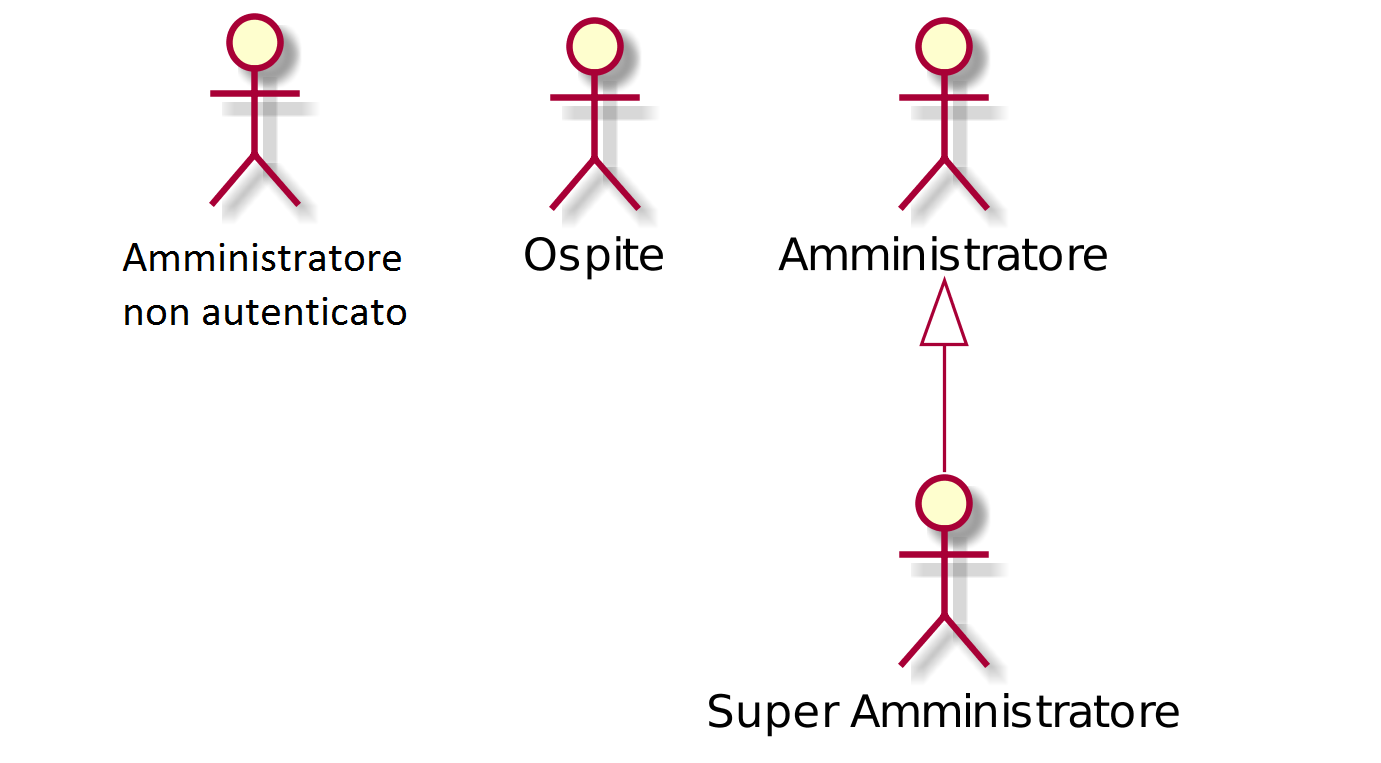
\includegraphics[scale=0.4]{images/Attori.png}
  \caption{Gerarchia degli attori}
\end{figure}
Dopo un'attenta analisi da parte del gruppo gli attori che sono stati individuati sono: 
\begin{itemize}
\item \textbf{Utente}: un utente del \gl{sistema}, il quale non è ancora stato identificato nè come amministratore nè come ospite;
\item \textbf{Ospite}: ospite esterno, il quale vuole incontrare un membro dell'azienda;
\item \textbf{Amministratore}: membro dell'azienda che dispone dei privilegi di amministrazione, i quali gli permettono di modificare il comportamento del sistema;
\item \textbf{Super Amministratore}: generalizzazione di amministratore, può creare e modificare altri amministratori e dispone di privilegi globali;
\end{itemize}
\newpage
\subsection{UC0: Funzionalità sistema}
\label{UC0}
\begin{figure}[h]
\centering
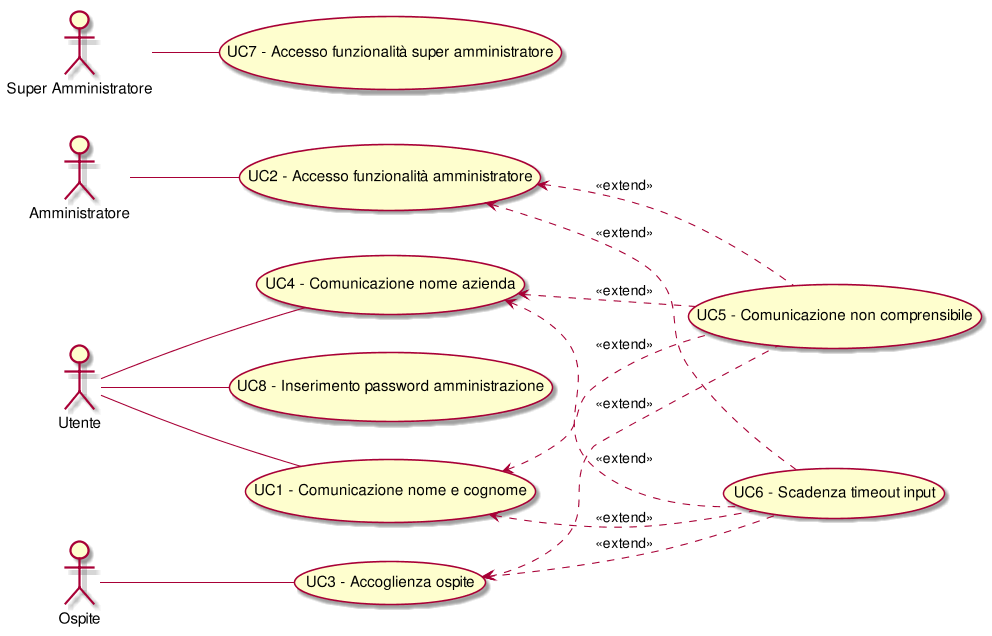
\includegraphics[width=\textwidth,height=\textheight,keepaspectratio]{images/UseCase.png}
\caption{UC0: Funzionalità sistema}
\end{figure}
\begin{longtable}{l|p{10cm}}
\rowcolor[gray]{0.8} \multicolumn{2}{c}{} \\
\rowcolor[gray]{0.8} \multicolumn{2}{c}{\textbf{UC0 - Funzionalità sistema}} \\
\rowcolor[gray]{0.8} \multicolumn{2}{c}{} \\
\hline
&\\
\textbf{Attori} & Utente, Amministratore, Super Amministratore, Ospite;\\[7pt]
\textbf{Descrizione} & Un utente deve poter fornire il proprio nome e cognome e l'azienda di provenienza. Nel caso in cui l'utente sia riconosciuto dal sistema come possibile amministratore (o super amministratore) deve poter fornire la propria password di amministrazione per accedere alle funzionalità a lui dedicate. Nel caso in cui si tratti di un ospite in visita, il sistema deve accoglierlo.\\[7pt]
\textbf{Precondizione} & Il sistema è avviato e pronto ad interagire con l'attore.\\[7pt]
\textbf{Postcondizione} & L'attore ha usufruito delle funzionalità desiderate offerte dal sistema. \\[7pt]
\textbf{Scenario principale} &
\begin{enumerate}
 \item L'utente può fornire il proprio nome e cognome;
 \item L'utente può fornire la propria azienda di provenienza;
 \item L'utente può fornire la propria password di amministrazione per accedere alle funzionalità di amministratore;
 \item L'ospite deve poter essere accolto tramite le funzionalità offerte dal sistema;
 \item L'amministratore può usufruire delle funzionalità di amministratore;
 \item Il super amministratore, oltre a quelle di amministratore, può usufruire di altre funzionalità dedicate al super amministratore.
\end{enumerate}
\\[7pt]\hline
\end{longtable}
\end{document}